%! Author = Sujal Singh
%! Date = 5/8/24

% Preamble
%! suppress = FileNotFound
\documentclass[11pt]{ipu-python}
\usepackage[
    pdftitle={Programming in Python Practical File},
    pdfsubject={Programming in Python Practical File},
    pdfauthor={Sujal Singh},
    pdfdisplaydoctitle,
    hidelinks,
]{hyperref}
\usepackage{tabularray}

% Packages
\usepackage{amsmath}
\usepackage{graphicx}

% Document
\makeindex
\begin{document}
    \maketitle
    % ---------------------------------------------------------------------------------------------------------------- %

    % ---------------------------------------------------------------------------------------------------------------- %
    \question{%
        Write a program to perform string maniuplation operations using set of pre-defined functions such as:
        \begin{itemize}
            \item find()
            \item upper()
            \item len()
            \item max() and min()
            \item fetching specific content from string
        \end{itemize}}\vspace*{10pt}
    \begin{code}
        {Program}{python}
string = "Hello, World!"

print(
    f'string: "{string}"\n',
    f'find("llo"): {string.find("llo")}',
    f'upper(): {string.upper()}',
    f'len(): {len(string)}',
    f'max(): "{max(string)}"',
    f'min(): "{min(string)}"',
    f'fetching "llo": "{string[(start := string.find("llo")):start + len("llo")]}"',
    sep="\n"
)
    \end{code}
    \begin{code}
        {Output}{text}
string: "Hello, World!"

find("llo"): 2
upper(): HELLO, WORLD!
len(): 13
max(): "r"
min(): " "
fetching "llo": "llo"
    \end{code}
    % ---------------------------------------------------------------------------------------------------------------- %

    % ---------------------------------------------------------------------------------------------------------------- %
    \\~\vfill%
    \question{%
        Write a program to test and check the mathematical functions such as:
        \begin{itemize}
            \item ciel()
            \item sqrt()
            \item pow()
            \item factorial()
        \end{itemize}}\vfill
    \newpage
    \begin{code}
        {Program}{python}
from math import ceil, sqrt, pow, factorial

num = 3.14

print(
    f"num: {num}\n",
    f"ceil(num): {ceil(num)}",
    f"sqrt(num): {sqrt(num)}",
    f"pow(num, 2): {pow(num, 2)}",
    f"factorial(5): {factorial(5)}",
    sep="\n"
)
    \end{code}
    \begin{code}
        {Output}{text}
num: 3.14

ceil(num): 4
sqrt(num): 1.772004514666935
pow(num, 2): 9.8596
factorial(5): 120
    \end{code}
    % ---------------------------------------------------------------------------------------------------------------- %

    % ---------------------------------------------------------------------------------------------------------------- %
    \\~\\%
    \question{Write a program that receives a number as input from user and returns if it's an odd or even number.}
    \begin{code}
        {Program}{python}
num = int(input("Enter an integer: "))
print(f"{num} is {'even' if num % 2 == 0 else 'odd'}.")
    \end{code}
    \begin{code}
        {Output}{text}
Enter an integer: 42
42 is even.
    \end{code}
    % ---------------------------------------------------------------------------------------------------------------- %

    % ---------------------------------------------------------------------------------------------------------------- %
    \\~\\
    \question{Write a program that receives input from the user to calculate the area of a triangle.}
    \begin{code}
        {Program}{python}
base = int(input("Enter base length of triangle(m): "))
height = int(input("Enter height of triangle(m): "))
print("area =", 0.5 * base * height)
    \end{code}
    \begin{code}
        {Output}{text}
Enter base length of triangle(m): 5
Enter height of triangle(m): 4
area = 10.0
    \end{code}
    \newpage
    % ---------------------------------------------------------------------------------------------------------------- %

    % ---------------------------------------------------------------------------------------------------------------- %
    \question{Write a program that receives input from the user to calculate the area of a square.}
    \begin{code}
        {Program}{python}
side = int(input("Enter side length of square(m): "))
print(f"Area of square of side length {side} is {side * side}.")
    \end{code}
    \begin{code}
        {Output}{text}
Enter side length of square(m): 4
Area of square of side length 4 is 16.
    \end{code}
    % ---------------------------------------------------------------------------------------------------------------- %

    % ---------------------------------------------------------------------------------------------------------------- %
    \\~\\
    \question{Write a program that receives input from the user to calculate the area of a rectangle.}
    \begin{code}
        {Program}{python}
length = int(input("Enter length: "))
breadth = int(input("Enter breadth: "))
print(f"Area of rectangle having length {length} and breadth {breadth} is {length * breadth}.")
    \end{code}
    \begin{code}
        {Output}{text}
Enter length: 5
Enter breadth: 4
Area of rectangle having length 5 and breadth 4 is 20.
    \end{code}
    % ---------------------------------------------------------------------------------------------------------------- %

    % ---------------------------------------------------------------------------------------------------------------- %
    \\~\\
    \question{Write a program to check if the input string is a palindrome or not.}
    \begin{code}
        {Program}{python}
original = input("Enter a string: ")
print("Given string is", "a" if original == original[::-1] else "not a", "palindrome.")
    \end{code}
    \begin{code}
        {Output}{text}
Enter a string: ehehe
Given string is a palindrome.
    \end{code}
    % ---------------------------------------------------------------------------------------------------------------- %

    % ---------------------------------------------------------------------------------------------------------------- %
    \question{Write a program that receives marks of a student for a subject as input and assigns a grade A$\|$B$\|$C%
        $\|$D$\|$E$\|$F.}
    \begin{code}
        {Program}{python}
offset = 9 - int(input("Enter marks for subject (0 - 100): ")) // 10
# Makes negative offset values equal zero
positive_offset = (abs(offset) + offset) // 2
print(chr(65 + positive_offset) if offset <= 5 else "F")
    \end{code}
    \begin{code}
        {Output}{text}
Enter marks for subject (0 - 100): 90
A
    \end{code}
    % ---------------------------------------------------------------------------------------------------------------- %

    % ---------------------------------------------------------------------------------------------------------------- %
    \question{Write a program to compute the GCD of two numbers.}
    \begin{code}
        {Program}{python}
def gcd(a, b):
    # Using the Euclidean algorithm
    if a < b:
        return gcd(a, b - a)
    elif a > b:
        return gcd(a - b, b)
    return a # if a equals b, then gcd is the same as a and b.


print(gcd(
    int(input("Enter first number: ")),
    int(input("Enter second number: "))
))
    \end{code}
    \begin{code}
        {Output}{text}
Enter first number: 10
Enter second number: 4
2
    \end{code}
    % ---------------------------------------------------------------------------------------------------------------- %

    % ---------------------------------------------------------------------------------------------------------------- %
    \\~\\
    \question{Write a program to check if the given number is an Armstrong number or not. Examples of Armstrong number
    are 153, 370, 371 etc.}
    \begin{code}
        {Program}{python}
num = int(str_num := input("Enter a number: "))

power = len(str_num)
print(
    "Given number is",
    "not an" if sum([int(digit) ** power for digit in str_num]) != num else "an",
    "Armstrong number."
)
    \end{code}
    \begin{code}
        {Output}{text}
Enter a number: 153
Given number is an Armstrong number.
    \end{code}
    % ---------------------------------------------------------------------------------------------------------------- %

    % ---------------------------------------------------------------------------------------------------------------- %
    \newpage
    \question{Write a program to check if the input year is a leap year or not.}
    \begin{code}
        {Program}{python}
from calendar import isleap

print(
    "Given year is",
    "a" if isleap(int(input("Enter a year: "))) else "not a",
    "leap year."
)
    \end{code}
    \begin{code}
        {Output}{text}
Enter a year: 2024
Given year is a leap year.
    \end{code}
    % ---------------------------------------------------------------------------------------------------------------- %

    % ---------------------------------------------------------------------------------------------------------------- %
    \\~\\
    \question{Write a program to compute factorial of a given number.}
    \begin{code}
        {Program}{python}
def fac(n):
    if n == 0:
        return 1
    return n * fac(n - 1)


print(fac(int(input("Enter a number: "))))
    \end{code}
    \begin{code}
        {Output}{text}
Enter a number: 5
120
    \end{code}
    % ---------------------------------------------------------------------------------------------------------------- %

    % ---------------------------------------------------------------------------------------------------------------- %
    \\~\\
    \question{Write a program to generate the Fibonacci sequence till 100.}
    \begin{code}
        {Program}{python}
a, b = 0, 1
print(a, end=" ")
while b <= 100:
    print(b, end=" ")
    a, b = b, b + a
    \end{code}
    \begin{code}
        {Output}{text}
0 1 1 2 3 5 8 13 21 34 55 89
    \end{code}
    \vfill
    % ---------------------------------------------------------------------------------------------------------------- %

    % ---------------------------------------------------------------------------------------------------------------- %
    \newpage
    \question{Write a program to print the multiplication table of a given number.}
    \begin{code}
        {Program}{python}
def table(n):
    for i in range(1, 11):
        print(f"{n} x {i} = {n * i}")


table(int(input("Enter a number: ")))
    \end{code}
    \begin{code}
        {Output}{text}
Enter a number: 3
3 x 1 = 3
3 x 2 = 6
3 x 3 = 9
3 x 4 = 12
3 x 5 = 15
3 x 6 = 18
3 x 7 = 21
3 x 8 = 24
3 x 9 = 27
3 x 10 = 30
    \end{code}
    % ---------------------------------------------------------------------------------------------------------------- %

    % ---------------------------------------------------------------------------------------------------------------- %
    \question{Write a program to create two lists and perform the following operation's:%
        \begin{enumerate}
            \item Add the elements of the two list.
            \item Compare the contents of the two list.
            \item Find the number of elements in the list.
            \item Sort the elements of the list.
            \item Reverse the contents of the list.
        \end{enumerate}}
    \begin{code}
        {Program}{python}
a, b = [1, 3, 2, 4, 5], [6, 5, 7, 9, 8]
print(
    [x + y for x, y in zip(a, b)],  # Only works for lists having same lengths
    a[2] == a[3],
    len(a), len(b),
    sorted(b),
    list(reversed(a)),
    sep="\n"
)
    \end{code}
    \newpage
    \begin{code}
        {Output}{text}
[7, 8, 9, 13, 13]
False
5
5
[5, 6, 7, 8, 9]
[5, 4, 2, 3, 1]
    \end{code}
    % ---------------------------------------------------------------------------------------------------------------- %

    % ---------------------------------------------------------------------------------------------------------------- %
    \question{Write a Program to create and display the content of the tuple. Initialize the tuple with the name of
    the cities. Display content of the tuple along with name/index positions of the cities.}
    \begin{code}
        {Program}{python}
cities = ("New Delhi", "Pune", "Jaipur", "Amritsar")
print(cities)
print(*[f"({i}): {name}" for i, name in enumerate(cities)], sep="\n")
    \end{code}
    \begin{code}
        {Output}{text}
('New Delhi', 'Pune', 'Jaipur', 'Amritsar')
(0): New Delhi
(1): Pune
(2): Jaipur
(3): Amritsar
    \end{code}
    % ---------------------------------------------------------------------------------------------------------------- %

    % ---------------------------------------------------------------------------------------------------------------- %
    \question{Write a program to create an array of even numbers till 14. Display the contents of array, compute the
    length of the array and also show how to delete a element from the desired position from the array.}
    \begin{code}
        {Program}{python}
array = list(range(0, 15, 2))
print(array)
print(len(array))
del array[3]
print(array)
    \end{code}
    \begin{code}
        {Output}{text}
[0, 2, 4, 6, 8, 10, 12, 14]
8
[0, 2, 4, 8, 10, 12, 14]
    \end{code}
    % ---------------------------------------------------------------------------------------------------------------- %

    % ---------------------------------------------------------------------------------------------------------------- %
    \question{Using \texttt{filter()} function, write a program to filter the elements which are greater than 9.}
    \begin{code}
        {Program}{python}
from random import randrange

data = [randrange(0, 20) for _ in range(20)]
print(list(filter(lambda x: x > 9, data)))
    \end{code}
    \newpage
    \begin{code}
        {Output}{text}
[12, 12, 17, 14, 15, 16, 12, 13, 11, 15, 14, 12]
    \end{code}
    % ---------------------------------------------------------------------------------------------------------------- %

    % ---------------------------------------------------------------------------------------------------------------- %
    \\~\\
    \question{Using \texttt{filter()} function, write a program to filter the elements which are greater than 9.}
    \begin{code}
        {Program}{python}
from random import randrange

data = [randrange(0, 100) for _ in range(30)]
print(data)
print(list(filter(lambda x: x % 5 == 0, data)))
    \end{code}
    \begin{code}
        {Output}{text}
[94, 39, 28, 55, 56, 39, 1, 53, 82, 24, 71, 20, 22, 36, 27, 40, 33, 67, 42, 94, 51, 41, 50, 3, 71, 15, 68, 29, 78, 79]
[55, 20, 40, 50, 15]
    \end{code}
    % ---------------------------------------------------------------------------------------------------------------- %

    % ---------------------------------------------------------------------------------------------------------------- %
    \\~\\
    \question{Write a program to create a file called “input.txt”, perform write/read operation on it with a string
    ``Computer Science''.}
    \begin{code}
        {Program}{python}
with open("input.txt", "w") as file:
    file.write("Computer Science")

with open("input.txt") as file:
    print(file.read())
    \end{code}
    \begin{code}
        {Output}{text}
Computer Science
    \end{code}
    % ---------------------------------------------------------------------------------------------------------------- %

    % ---------------------------------------------------------------------------------------------------------------- %
    \\~\\
    \question{Write a program to create a file called “input.txt”, initialize it with a string of your choice and
    perform the read operation to read only the first 3 characters from the file.}
    \begin{code}
        {Program}{python}
with open("input.txt", "w") as file:
    file.write("Hello, World!")

with open("input.txt") as file:
    print(file.read(3))
    \end{code}
    \begin{code}
        {Output}{text}
Hel
    \end{code}
    \newpage
    % ---------------------------------------------------------------------------------------------------------------- %

    % ---------------------------------------------------------------------------------------------------------------- %
    \question{Using NumPy, write a program to create 1-dimensional array, load it with numbers, and perform the
    operation of iteration and slicing on it.}
    \begin{code}
        {Program}{python}
import numpy as np

print(arr := np.array([2, 3, 4, 1, 7, 6], np.int32))
for e in np.nditer(arr):
    print(e, end=" ")
print()
print(arr[2:5])
    \end{code}
    \begin{code}
        {Output}{text}
[2 3 4 1 7 6]
2 3 4 1 7 6
[4 1 7]
    \end{code}
    % ---------------------------------------------------------------------------------------------------------------- %

    % ---------------------------------------------------------------------------------------------------------------- %
    \\~\\
    \question{Using NumPy, write a program to create multidimensional array, load it with the numbers and display the
    content of it.}
    \begin{code}
        {Program}{python}
import numpy as np

arr = np.array([[1, 2, 3], [4, 5, 6]])
print(arr)
    \end{code}
    \begin{code}
        {Output}{text}
[[1 2 3]
 [4 5 6]]
    \end{code}
    % ---------------------------------------------------------------------------------------------------------------- %

    % ---------------------------------------------------------------------------------------------------------------- %
    \\~\\
    \question{Using NumPy, write a program to create two 1-dimensional array and perform the operation of iteration,
        sorting the contents of array and concatenating the contents of the array.}
    \begin{code}
        {Program}{python}
import numpy as np

arr = np.array([9, 4, 6, 2, 7])

for e in np.nditer(arr):
    print(e)

print(np.sort(arr))
print(np.concatenate((arr, np.array([38, 77, 29, 84, 75]))))
    \end{code}
    \begin{code}
        {Output}{text}
9
4
6
2
7
[2 4 6 7 9]
[ 9  4  6  2  7 38 77 29 84 75]
    \end{code}
    % ---------------------------------------------------------------------------------------------------------------- %

    % ---------------------------------------------------------------------------------------------------------------- %
    \\~\\
    \question{Using NumPy, initialize an array and display its dimensionality.}
    \begin{code}
        {Program}{python}
import numpy as np

arr = np.array([[[1, 2], [3, 4]], [[5, 6], [6, 7]], [[8, 9], [9, 10]]])
print(arr.shape)
    \end{code}
    \begin{code}
        {Output}{text}
(3, 2, 2)
    \end{code}
    % ---------------------------------------------------------------------------------------------------------------- %

    % ---------------------------------------------------------------------------------------------------------------- %
    \\~\\
    \question{Using Pandas, create a dataframe, initialize it with the contents such as your enrollment Number and
    name and display them.}
    \begin{code}
        {Program}{python}
import numpy as np
import pandas as pd

class_list = pd.DataFrame(np.array([
    ["Name", "Enrollment Number"],
    ["Alice", 1],
    ["Bob", 2],
    ["Bob", 3]
]))

print(class_list)
    \end{code}
    \begin{code}
        {Output}{text}
       0                  1
0   Name  Enrollment Number
1  Alice                  1
2    Bob                  2
3    Bob                  3
    \end{code}
    % ---------------------------------------------------------------------------------------------------------------- %

    % ---------------------------------------------------------------------------------------------------------------- %
    \newpage
    \question{Create 2 arrays, using MatPlotLib, plot the graph with the content of the two arrays, with coordinates
    plotted on x-axis and y-axis.}
    \begin{code}
        {Program}{python}
import numpy as np
import matplotlib.pyplot as plt

plt.plot(
    np.array([np.random.randint(0, 100) for _ in range(50)]),
    np.array([np.random.randint(0, 100) for _ in range(50)]),
    "ko"
)
plt.show()
    \end{code}
    \outputfigure[0.35]{figures/q27}
    % ---------------------------------------------------------------------------------------------------------------- %

    % ---------------------------------------------------------------------------------------------------------------- %
    \question{Create a .csv file (with contents like age, weight and BMI). Read the content of the file and using
    Pandas and MatPlotLib, plot the graph.\\}
    \noindent\hspace{-5pt}%
    \begin{tblr}{colspec={|X[1,c]|X[1,c]|X[1,c]|X[1,c]|},hlines,vlines}%
        \SetCell[c=4]{c} \textbf{\large data.csv} \\
        \textbf{Age} & \textbf{Height} & \textbf{Weight} & \textbf{BMI} \\
        21           & 185             & 109             & 31.84        \\
        47           & 173             & 74              & 4.72         \\
        46           & 174             & 78              & 5.76         \\
        34           & 171             & 66              & 2.57         \\
        33           & 174             & 76              & 5.10         \\
    \end{tblr}\\[10pt]
    \begin{code}
        {Program}{python}
import pandas as pd
import matplotlib.pyplot as plt

data = pd.read_csv("data.csv")

fig, ax = plt.subplots(subplot_kw={"projection": "3d"})
ax.plot(data["Weight"], data["Height"], data["BMI"], "ko")

plt.show()
    \end{code}
    \newpage\vspace*{-20pt}
    \noindent\textbf{Output:}
    \begin{center}
        \hspace{-0.1\linewidth}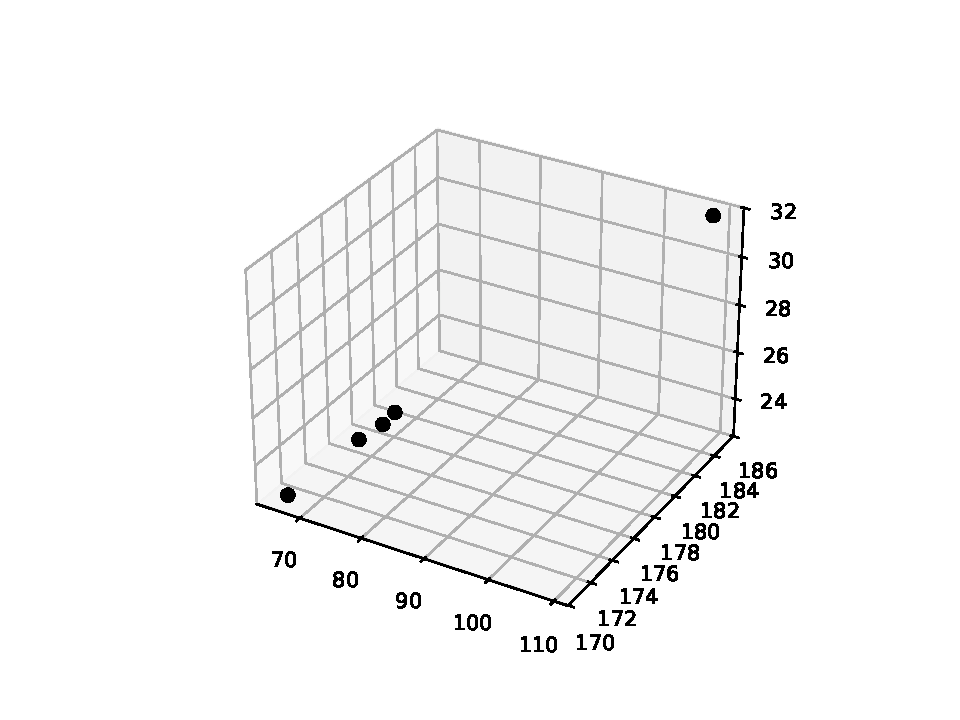
\includegraphics[width=0.9\linewidth]{figures/q28}
    \end{center}
    % ---------------------------------------------------------------------------------------------------------------- %

    % ---------------------------------------------------------------------------------------------------------------- %
    \question{Create a .csv file (with contents like age, weight and BMI). Read the content of the file and using
    Pandas and MatPlotLib, plot the histogram.}
    \begin{code}
        {Program}{python}
import numpy as np
import pandas as pd
import matplotlib.pyplot as plt

data = pd.read_csv("data.csv")

bmi = data["BMI"]
grp_size = 2
average_group_bmi = np.array([
    sum(bmi[i:i + grp_size]) / grp_size
    for i in range(0, len(bmi), grp_size)
])

bins = data["Age"][0:len(data["Age"]):grp_size]
plt.hist(bins[:-1], bins, weights=average_group_bmi[:-1], fill=False)

plt.show()
    \end{code}
    \newpage
    \outputfigure[0.5]{figures/q29}
    % ---------------------------------------------------------------------------------------------------------------- %

    % ---------------------------------------------------------------------------------------------------------------- %
    \question{Write a program to create a class called ``Student'' with fields such as: Enrollment Number, USS Name,
        Branch Name, Student Name, etc. Instantiate a class and make a call to user defined function to display the
        details of students.}
    \begin{code}
        {Program}{python}
class Student:
    def __init__(self, enrollment_number, uss, branch, name):
        self.enrollment_number = enrollment_number
        self.uss = uss
        self.branch = branch
        self.name = name

    def display(self):
        print(
            f"Name: {self.name}",
            f"Enrollment Number: {self.enrollment_number}",
            f"Branch: {self.branch}",
            f"USS: {self.uss}",
            sep="\n"
        )


Student("04119051723", "USAR", "IIOT", "Sujal Singh").display()
    \end{code}
    \begin{code}
        {Output}{text}
Name: Sujal Singh
Enrollment Number: 04119051723
Branch: IIOT
USS: USAR
    \end{code}
    % ---------------------------------------------------------------------------------------------------------------- %

    % ---------------------------------------------------------------------------------------------------------------- %
    \newpage
    \question{Write a program to create a class called ``Student'' with fields such as: Enrollment Number, USS Name,
        Branch Name, Student Name, etc. Instantiate a class and make a call to user defined function to display the
        details of students.}
    \begin{code}
        {Program}{python}
class Employee:
    def __init__(self, emp_id, name):
        self.emp_id = emp_id
        self.name = name

    def display(self):
        print(f"Name: {self.name}\nID: {self.emp_id}")


Employee("04119051723", "Sujal Singh").display()
    \end{code}
    \begin{code}
        {Output}{text}
Name: Sujal Singh
ID: 04119051723
    \end{code}
    % ---------------------------------------------------------------------------------------------------------------- %
\end{document}